
\documentclass[a4paper,11pt]{article}

\usepackage[top=2.25cm, bottom=2.25cm, left=2.25cm, right=2.25cm]{geometry}

\usepackage[pdftex]{graphicx}
\pdfsuppresswarningpagegroup=1
\usepackage{tikz}
\usetikzlibrary{shapes, arrows, arrows.meta}

\usepackage{array}
\usepackage{longtable} 
\usepackage{booktabs}

\usepackage{amsfonts,amstext,amscd,bezier,amsthm,amssymb}
\usepackage[centertags]{amsmath}

\usepackage{mathtools}
\usepackage[utf8]{inputenc} 
\usepackage[T1]{fontenc}

\usepackage[sort]{natbib}

\usepackage[french]{babel} 
\NoAutoSpaceBeforeFDP
\usepackage{subcaption}

\usepackage{kpfonts}

\usepackage{color}
\definecolor{darkgreen}{rgb}{0,0.5,0}
\definecolor{darkmagenta}{rgb}{0.5,0,0.5}
\definecolor{darkgray}{rgb}{0.5,0.5,0.5}
\definecolor{darkblue}{rgb}{0.2,0.2,0.4}
\definecolor{darkred}{rgb}{0.6,0.15,0.15}
\definecolor{gray}{rgb}{0.65,0.65,0.65}
\definecolor{lightgray}{rgb}{0.8,0.8,0.8}
\definecolor{lightblue}{rgb}{0.5,0.5,1}
\definecolor{lightgreen}{rgb}{0.5,1,0.5}
\definecolor{deadred}{rgb}{0.7, 0.2, 0.2}
\definecolor{deadblue}{rgb}{0.2, 0.2, 0.7}

\usepackage{icomma}
\usepackage{url}
\usepackage[hidelinks]{hyperref}
\usepackage{enumitem} 

\usepackage[ruled, vlined, french, onelanguage]{algorithm2e}

\usepackage{pdflscape}

\usepackage{cleveref}

\captionsetup[subfigure]{subrefformat=simple,labelformat=simple}
\renewcommand\thesubfigure{(\alph{subfigure})}

\theoremstyle{plain}
\newtheorem*{prop}{Proposition}
\theoremstyle{definition}
\newtheorem*{defi}{Définition}
\newtheorem*{remk}{Remarque}
\newcommand\norm[1]{\left\lVert#1\right\rVert}

\DeclarePairedDelimiter{\ceil}{\lceil}{\rceil}
\DeclarePairedDelimiter{\floor}{\lfloor}{\rfloor}
\DeclarePairedDelimiter{\abs}{\lvert}{\rvert}
\DeclareMathOperator*{\argmax}{argmax}
\DeclareMathOperator*{\argmin}{argmin}
\DeclareMathOperator{\ECO}{ECO}
\DeclareMathOperator{\ECR}{ECR}
\DeclareMathOperator{\EC}{EC}
\DeclareMathOperator{\EVOI}{EVOI}

\renewcommand\floatpagefraction{.9}
\renewcommand\topfraction{.9}
\renewcommand\bottomfraction{.9}
\renewcommand\textfraction{.1}
\setcounter{totalnumber}{50}
\setcounter{topnumber}{50}
\setcounter{bottomnumber}{50}

\begin{document}

\setlist[itemize]{label=\textbullet, nosep}


\pagestyle{plain}

\title{ML : Rapport des TMEs}
\author{Ivan Kachaikin}
\date{}
\maketitle


\section{Introduction}
Ce document représente le rapport des TMEs effectués pour l'UE ML. Chacune de ses sections correspond à l'une de 4 TMEs répondant aux questions y posées.

\section{TME 1 : Arbres de décisions}
\label{tme1}
Le but principal de ce TME était d'implémenter un classificateur binaire qui se fonde sur les arbres de décision. L'on remarque que toutes les questions pour lesquelles il n'y a pas de réponses dans ce rapport consistaient à coder telle ou telle mécanisme concrète, et alors on ne les inclut pas.

\textbf{Q 1.3.} Après avoir lancé des calculs de différences demandée, on constate que pour les données fournies ``Drama'' est un attribut à partir duquel on doit commencer car cela nous donne un gain d'information le plus haut égal à 0.073671. On remarque qu'une valeur 0 de l'entropie correspond au cas où il n'y a pas des aspects aléatoires tandis qu'une valeur 1 correspond bien au désordre le plus grand (lorsqu'on a une variable binaire et lorsqu'on prend le log de base 2). Alors, se retournant au gain d'information, des valeurs plus hauts correspondent au cas où le désordre pour des valeurs de l'attribut est plus grand alors que le désordre pour y est minimal. Et cela c'est ce qu'on cherche : un attribut dont les valeurs sont les plus 
``équilibrées'' mais qui produisent les étiquettes les plus ``claires''.

\textbf{Q 1.4.} Sur la base de données imdb, l'on a construit certains arbres des profondeurs différentes qui appartiennent à l'ensemble $\{5, 10, 15, 20, 25\}$. L'on constate que plus est la profondeur plus d'exemples l'on sépare. Généralement, ce comportement semble normal car à chaque fois que l'on va plus ``loin'' dans un arbre, on sépare encore plus des exemplaires.

\textbf{Q 1.5.} Les scores sont fournis dans une Figure~\ref{TreeScoreEvolution} ci-dessous créé par \texttt{matplotlib.pyplot}. L'on observe qu'un score de bonne classification plus élevé correspond à une profondeur de plus grande valeur. Un tel résultat est plutôt attendu parce que si la profondeur est plus grande alors l'on peut séparer mieux des exemplaires. Donc on peut dire que c'est plutôt normal. En revanche, l'on remarque qu'une croissance de score ralentit dès qu'une profondeur augmente donc l'évolution de score est une fonction concave.

\begin{figure}[ht]
\centering
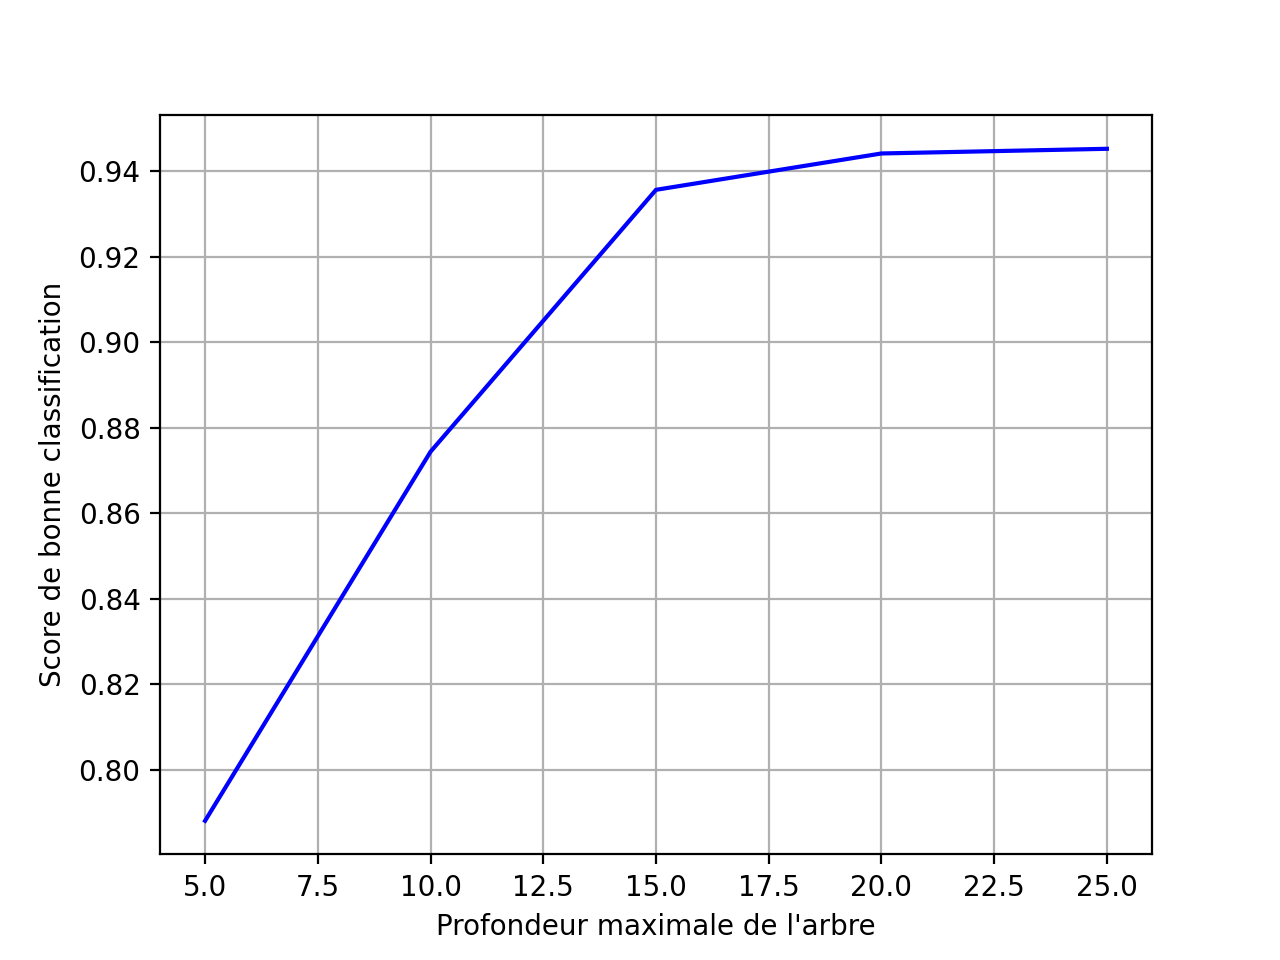
\includegraphics{Figures/Figure_0.png}
\caption{Évolution de score de la bonne classification en fonction de la profondeur maximale permise de l'arbre}
\label{TreeScoreEvolution}
\end{figure}

\textbf{Q 1.6.} En fait, le score ne peut pas être un indicateur fiable du comportement parce que cela nous dit tout simplement que l'algorithme marche bien pour les données fournies en entrée. Par contre, il n'y a aucune garantie que cela marcherait pour les autres données pas encore observées. Une approche assez classique pour résoudre ce problème-là c'est de séparer une base de données initiale en deux : celle qu'on utilise pour apprendre le modèle et celle d'autre que l'on n'utilise pas pendant l'apprentissage mais que l'on utiliserait pour tester le modèle obtenu. Suivant une telle méthode, notre but serait de minimiser l'erreur d'apprentissage et celle liée au test.

\textbf{Q 1.7.} Une réponse est donnée par la Figure~\ref{TreeErrorEvolution} ci-dessous.

\begin{figure}[ht]
    \begin{subfigure}{.5\textwidth}
    	\centering
    	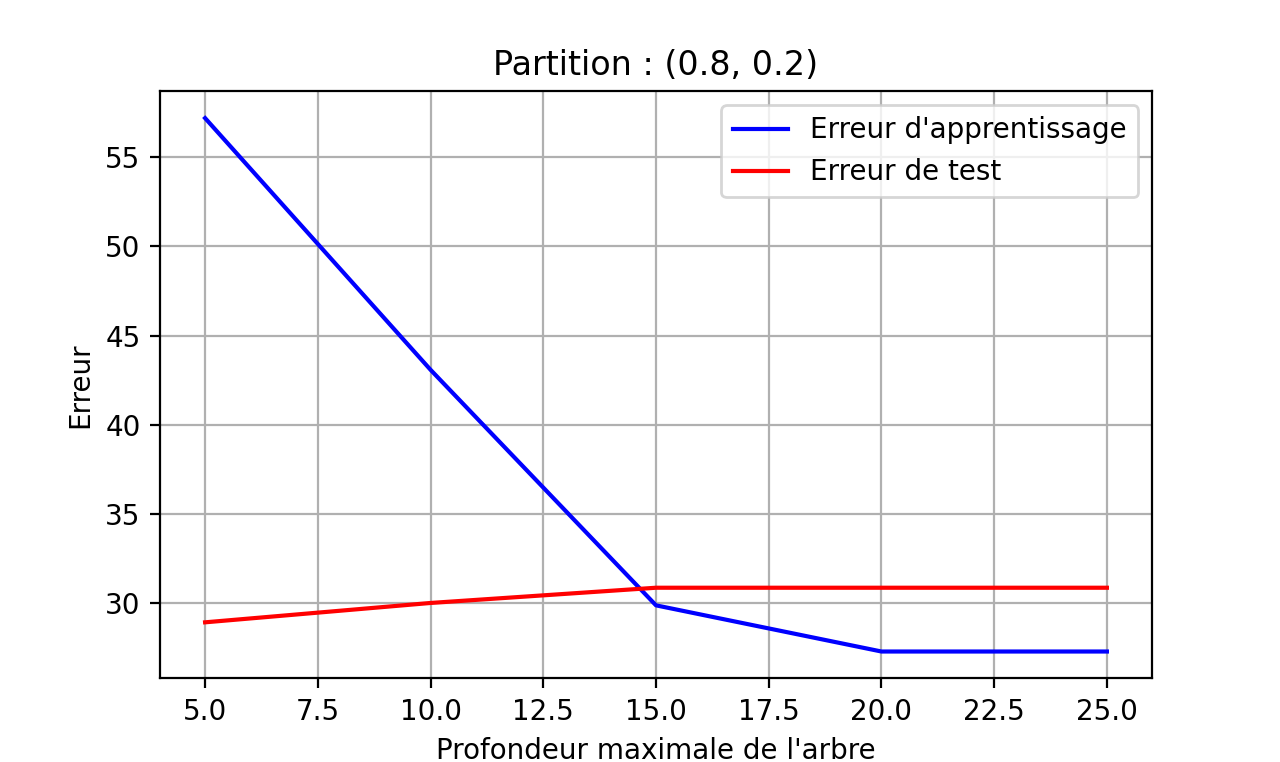
\includegraphics{Figures/Figure_1.png}
    \end{subfigure}
    
    \begin{subfigure}{.5\textwidth}
    	\centering
    	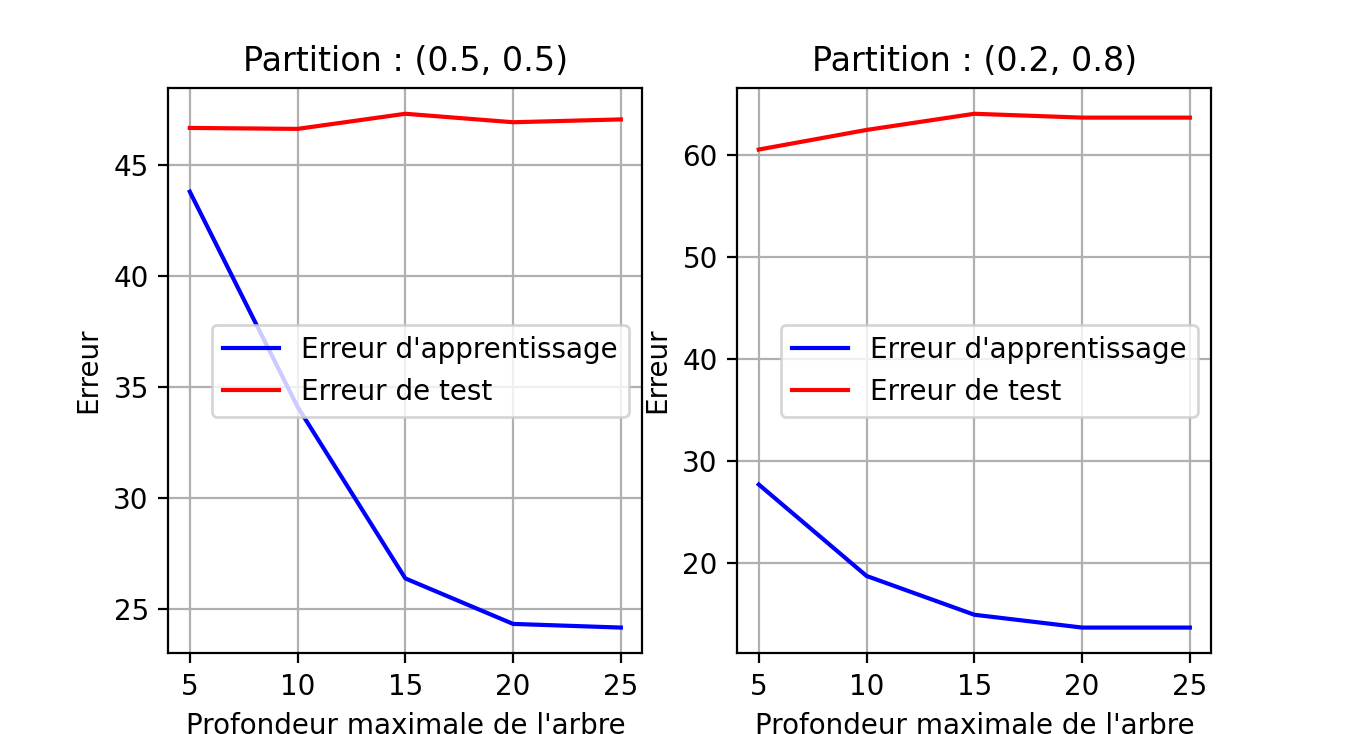
\includegraphics{Figures/Figure_2.png}
    \end{subfigure}
\caption{Évolution de l'erreur en fonction de la profondeur étant donné des partitions différentes}
\label{TreeErrorEvolution}
\end{figure}

\textbf{Q 1.8.} L'on constate que quand il y a peu d'exemples d'apprentissage l'erreur d'apprentissage devient la plus petite, en revanche, cela produit l'erreur de test la plus élevée (sur-apprentissage). Pour ce cas-là, tel comportement n'est pas trop inattendue parce que, intuitivement, moins est une taille de données en entrée, plus facile il est pour le modèle de s'adapter pour ces données. D'autre part, tel modèle n'est ajusté que pour le nombre d'exemples assez petit ne peut pas être capable à marcher proprement pour les données pas utilisées pendant l'apprentissage. L'on observe un résultat assez pareil si les partitions ont des quantités égales des exemplaires. Pour le cas inverse où la majorité d'exemples sont ceux d'apprentissage, on observe des résultats bien différents. En fait, l'erreur d'apprentissage est la plus élevée par rapport à ces trois partitionnements, par contre, cela nous donne la meilleure l'erreur de test. Il existe, de plus, pour ce cas un point 15 pour lequel deux erreur prennent presque les mêmes valeurs. Ce point est un bon compromis entre sous-apprentissage et sur-apprentissage. Par conséquent, l'on pourrait considérer le modèle correspondant à ce point-là comme celui le meilleur.

\textbf{Q 1.9.} Une stabilité des résultats obtenus est une question assez discutable. D'un côté, on constate que le modèle concerné fait assez beaucoup de classifications fautes pour tous les partitionnement, de l'autre côté , cela peut suffire pour les cas particulières où l'exactitude complète n'est pas nécessaire. Par rapport aux améliorations possibles, l'idée de base est de modifier une façon selon laquelle on représente les données. Tout d'abord, cela peut être utile de les normaliser. Ensuite, on pourrait utiliser telle ou telle approche pour extraire des caractéristiques relativement pas principales pour ne pas les considérer pendant une classification. Finalement, on peut utiliser les autres algorithmes de classification pour voir comment cette approche marche par rapport à d'autres.

\textbf{Questions de bonus.} Après avoir relancé des simulations utilisant une validation croisée l'on constate que l'erreur la plus petite de valeur 12.873 correspond au nombre de partitions le plus grand qui était 25 (parmi $\{5, 10, 15, 20, 25\}$). D'autre côté, la profondeur n'était pas maximale et a eu une valeur de 10 (parmi $\{5, 10, 15, 20, 25\}$) ce qui est assez intéressant car on attendait plutôt que plus est la profondeur, moins est l'erreur.


\section{TME 2 : Estimation de densité}
\label{tme2}

Dans le cadre de ce TME, l'on a eu pour but d'estimer la densité d'une variable aléatoire multidimensionnelle $X$ étant donné son échantillon. C'est pour cette raison que l'on a implémenté deux techniques qui permettent de résoudre un tel problème :
\begin{itemize}
    \item méthode des histogramme ;
    \item méthode à noyaux.
\end{itemize}
Pour réaliser ces deux approches concernées, l'on a développé un module \texttt{DensityEstimationModel.py} qui contient principalement des éléments suivants:
\begin{itemize}
    \item \texttt{DensityEstimationModel} : une classe qui représente un modèle de l'estimation de la densité ;
    \item \texttt{histogram} et \texttt{kernel} : fonctions avec presque la même interface qui crée le modèle de l'estimation correspondant à leurs noms ;
    \item certaines méthodes auxiliaire, particulièrement, deux noyaux prédéfinis (fenêtre de Parzen et gaussienne).
\end{itemize}
Tous les éléments de ce module sont bien documentés, alors pour les raisons spatiales l'on évite les détails ici.

Les estimations obtenues par les techniques implémentées avec \texttt{POI = night\_club} sont données dans la Figure~\ref{DensEstim}. L'on remarque que toutes les méthodes conçues admettent le cas où $\text{dim}(X) > 2$. L'on note également que c'est bien possible d'utiliser des noyaux définis par l'utilisateur.

\begin{figure}[ht]
    \centering
    \begin{subfigure}{1.0\textwidth}
    	\centering
    	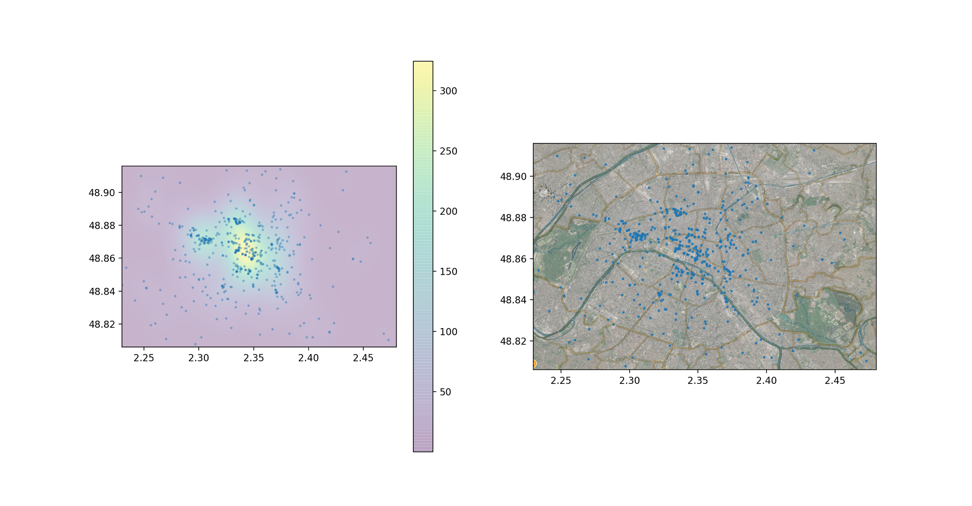
\includegraphics{Figures/Figure_3.png}
    	\caption{}
    	\label{DensEstimKernelGauss}
    \end{subfigure}

    \begin{subfigure}{1.0\textwidth}
    	\centering
    	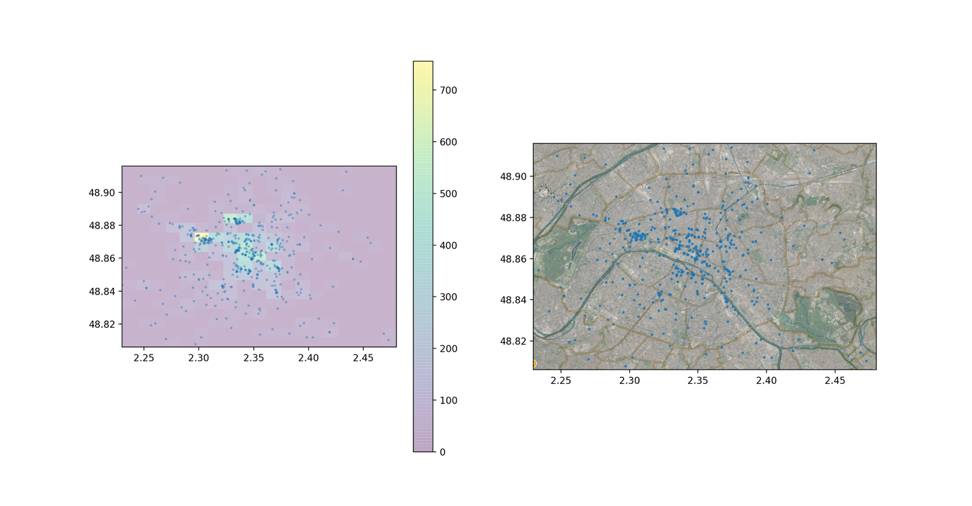
\includegraphics{Figures/Figure_4.png}
    	\caption{}
    	\label{DensEstimHist20}
    \end{subfigure}
    \caption{Estimation par noyau (gausienne) -- (a), estimation par histogramme avec une taille de grille égal à 20 -- (b)}
    \label{DensEstim}
\end{figure}

\textbf{Q 2.1.} Pour une faible discrétisation la méthode des histogrammes n'est pas assez précise car dans ce cas-là une case dans une grille devient trop grand. C'est bien possible alors d'y avoir une région avec une concentration des points, et l'une autre sans aucun point. Mais comme ces deux régions hypothétiques appartiendraient à une seule case, l'on estimerait leurs densités comme celles de mêmes valeurs tandis que c'est bien évident que la densité est différent pour ces deux régions.

En revanche, pour une discrétisation trop forte l'on peut obtenir des cases qui sont trop petites. C'est pourquoi c'est très probable pour ce cas d'avoir la densité qui se ressemble à une fonction de Dirac avec des valeurs très grandes dans les points d'échantillon considéré, en même temps ayant à peu près 0 pour tous les autres points.

Par conséquent, la question de choix de pas de la discrétisation n'est pas triviale, et il faut trouver un bon compromis pour obtenir le modèle suffisant.

\textbf{Q 2.2.} Rôle des paramètres dans la méthode à noyau dépend de noyau particulier utilisé puisque chaque noyau prend son propre ensemble des paramètres. À l'inverse, chacune telle méthode suppose une constance de la densité autour du point où l'on calcule cette densité. Alors, toutes les méthodes à noyau prennent pour un paramètre une valeur $h_n$ qui est une longueur de l'hypercube où la densité ne change pas.

\textbf{Q 2.3-2.4.} Une première approche plutôt théorique consiste à trouver des meilleurs paramètres / évaluer la qualité du modèle par maximum de vraisemblance : l'on choisit tels paramètres qui maximise une valeur de log-vraisemblance, ensuite, pour les paramètres déjà connus l'on peut analyser le modèle obtenu en calculant une vraisemblance d'avoir pour telles données une telle densité avec ces paramètres donnés.

\section{TME 3 : Descente de gradient, perceptron}
\label{tme3}

\textbf{Q 3.1.} L'on a implémenté tout le code demandé : l'on a définit des fonctions pour calculer des erreurs ainsi que leurs gradients, l'on a rempli une classe \texttt{Lineaire} ajoutant la prise en compte de biais et permettant à l'utilisateur de choisir une mode de fonction \texttt{fit} (``batch'', ``sgd'' ou ``mini-batch''). De plus, l'on a réalisé également une technique du choix dynamique de ``learning rate'' en utilisant la méthode de Barzilai–Borwein :

\begin{equation}
    \gamma_n = \frac{\mid (\text{\textbf{w}}_n - \text{\textbf{w}}_{n-1})^T (\nabla E(\text{\textbf{w}}_n) - \nabla E(\text{\textbf{w}}_{n-1}))) \mid}{\norm{\nabla E(\text{\textbf{w}}_n) - \nabla E(\text{\textbf{w}}_{n-1})}^2}
\end{equation}
où une formule de descente de gradient était la suivante :

\begin{equation}
    \text{\textbf{w}}_{n+1} = \text{\textbf{w}}_n - \gamma_n \nabla E(\text{\textbf{w}}_n)
\end{equation}

Cette modification nous permet d'accélérer les calculs car l'on atteint plus vite au point d'optimum. Par contre, de temps en temps son utilisation nous retourne des solutions qui ne sont pas admissibles.

Les résultats d'apprentissage (trajectoire d’apprentissage et des frontières) du perceptron et de la régression sont données dans la Figure~\ref{PercRegrRes}.

\begin{figure}
    \centering
    \begin{subfigure}{1.0\textwidth}
    	\centering
    	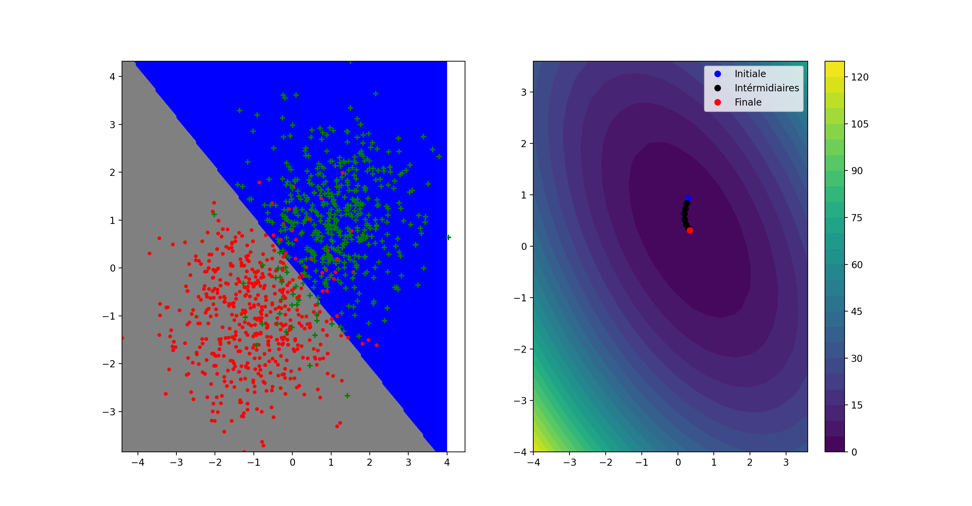
\includegraphics{Figures/Figure_5.png}
    	\caption{}
    	\label{RegressionSimpleRes}
    \end{subfigure}

    \begin{subfigure}{1.0\textwidth}
    	\centering
    	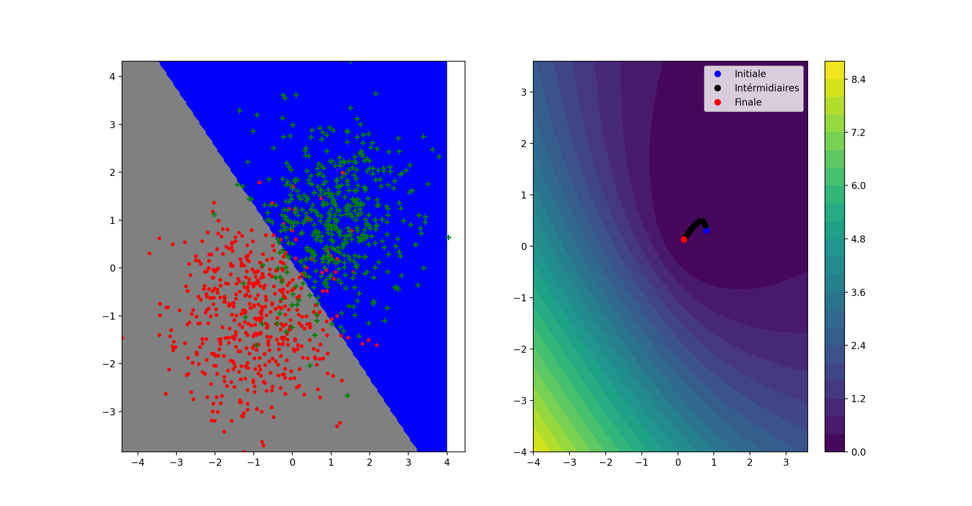
\includegraphics{Figures/Figure_6.png}
    	\caption{}
    	\label{PercSimpleRes}
    \end{subfigure}
    \caption{Les résultats d'apprentissage des modèles linéaires obtenus avec la descente de gradient par ``mini-batch'' : (a) -- Régression, (b) -- Perceptron}
    \label{PercRegrRes}
\end{figure}

\textbf{Q 3.2.} Afin que le perceptron puisse comparer 2 chiffres (6 vs. 9) parmi 10, on a utilisé une base de données raccourcie. Tout d'abord, l'on a récupéré les données pour lesquelles une valeur d'étiquettes est 6 ou 9, ensuite, l'on a remplacé dans ces nouvelles données tous les labels 6 par 1 et 9 par -1. Pour le cas où l'on voudrait comparer une chiffre avec toutes les autres l'on a fait de même façon sauf que l'on a utilisé une base de données complète. Les scores de bonne classification ont été les suivants :

\begin{itemize}
    \item \textbf{6 vs. 9} : 99.8\% pour apprentissage, 98.6\% pour test ;
    \item \textbf{6 vs. les autres} : 98.2\% pour apprentissage, 97.5\% pour test.
\end{itemize}
Les autres résultats sont fournis dans la Figure~\ref{ResUSPS} où l'on trace des matrices de poids (à gauche) et l'évolution des erreurs (à droite). Observant des matrices, l'on constate que les poids ont des valeurs plutôt négatives dans les régions où les classes ont des similarités, et de valeurs plutôt positives sinon. Analysant des erreurs et de scores de bonne classification, l'on peut résumer qu'il existe une très légère sur-apprentissage dans un modèle considéré. Pourtant, l'on suppose que cette différence est trop petite pour être signifiante.

\begin{figure}
    \centering
    \begin{subfigure}{1.0\textwidth}
    	\centering
    	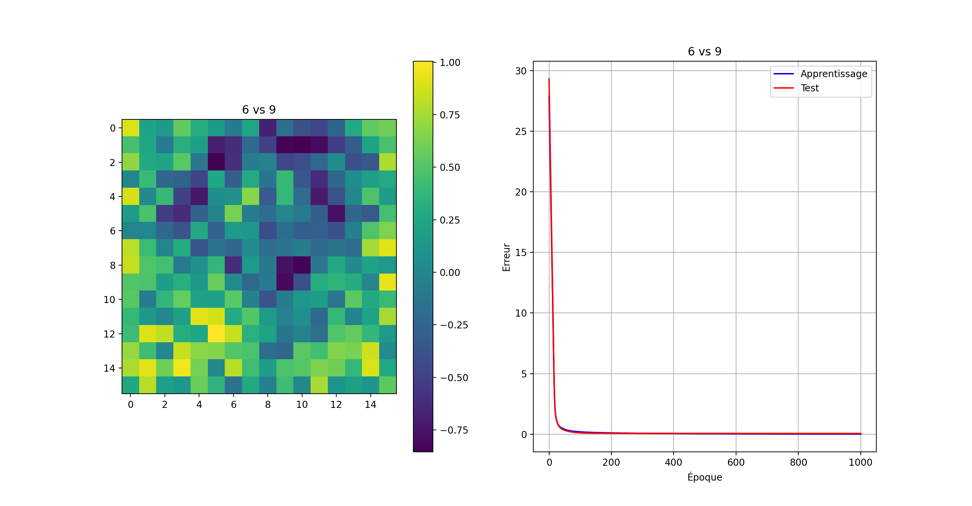
\includegraphics{Figures/Figure_7.png}
    	\caption{}
    	\label{ResUSPS6vs9}
    \end{subfigure}

    \begin{subfigure}{1.0\textwidth}
    	\centering
    	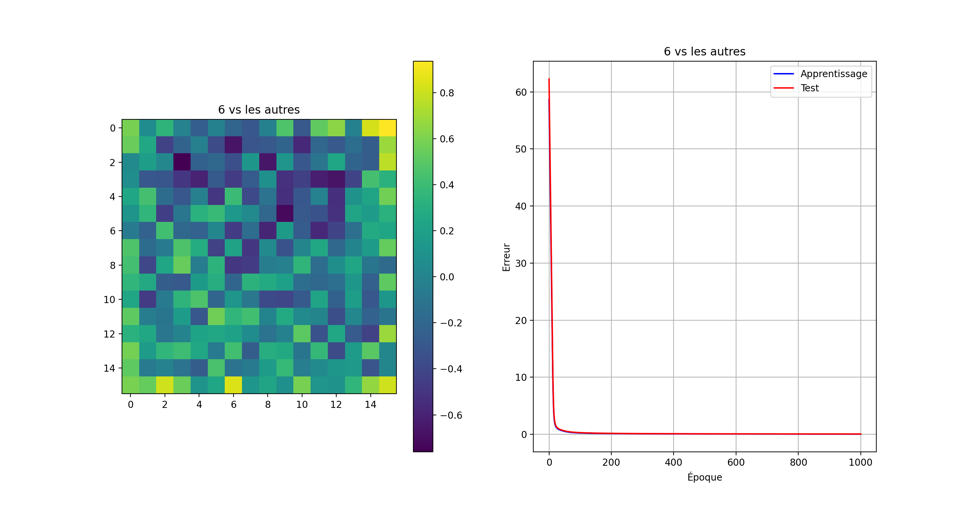
\includegraphics{Figures/Figure_8.png}
    	\caption{}
    	\label{ResUSPS6vsOther}
    \end{subfigure}
    \caption{Les résultats obtenus pour l'apprentissage effectuée sur la base de données \texttt{USPS} ; (a) -- \textbf{6 vs. 9}, (b) -- \textbf{6 vs. les autres}}
    \label{ResUSPS}
\end{figure}

\textbf{Q 3.3.} Bien qu'à l'avant des modèles linéaires aient marché bien pour les données artificielle, générant un autre type de données passant, par exemple, \texttt{data\_type=1} l'on n'aurait plus de capacité à classifier proprement ni avec le perceptron, ni avec la régression non plus. C'est pour cette raison que l'on lance des projections. Plus précisément, l'on a implémenté une projection polynomiale ainsi que celle gaussienne ce qui nous permettait d'améliorer notre classificateur pour le cas où les classes considérées ne sont pas séparables linéairement. En effet, en termes des scores l'on a obtenu pour les modèles linéaires :

\begin{itemize}
    \item Perceptron : précisément 50\%  pour apprentissage, 49.8\%  pour test ;
    \item Régression : 52.1\% pour apprentissage, 50.9\% pour test.
\end{itemize}
En même temps, pour les modèles projetés l'on a reçu :

\begin{itemize}
    \item Projection polynomiale : 98.7\%  pour apprentissage, 97.6\%  pour test ;
    \item Projection gaussienne : 91.7\% pour apprentissage, 66.7\% pour test.
\end{itemize}
Des frontières de séparation sont indiquées dans la Figure~\ref{PolyGaussProjection}.

Pour conclure, l'on constate que la projection comparant aux modèles linéaires nous permet de faire face aux problèmes de classifications où les classes ne sont pas séparables linéairement. De plus, l'on remarque la projection polynomiale, quadratique plus spécifiquement, a été plus efficace que celle gaussienne. Par contre, l'on suppose qu'il existe tels paramètres de la projection gaussienne qui lui permettent d'être aussi efficace.

\begin{figure}
    \centering
    \begin{subfigure}{1.0\textwidth}
    	\centering
    	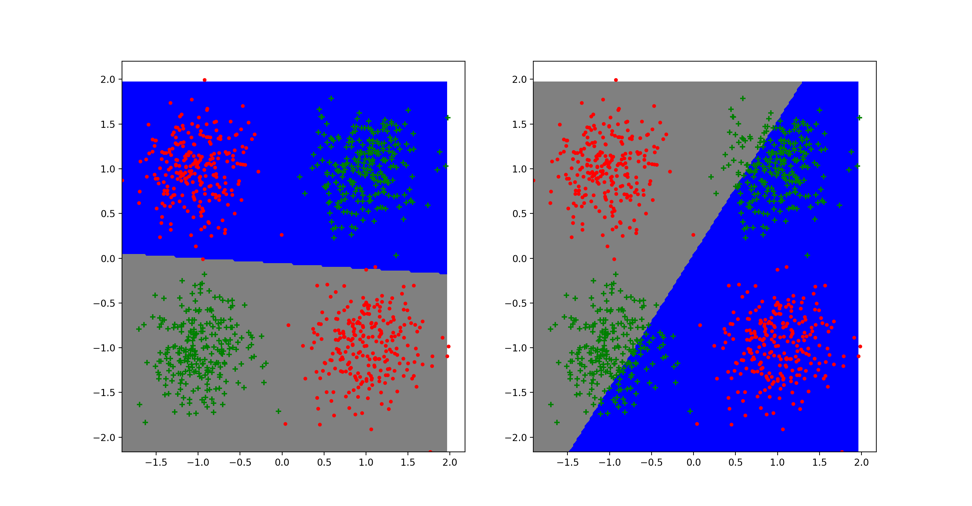
\includegraphics{Figures/Figure_9.png}
    	\caption{}
    	\label{WithoutProjection}
    \end{subfigure}

    \begin{subfigure}{1.0\textwidth}
    	\centering
    	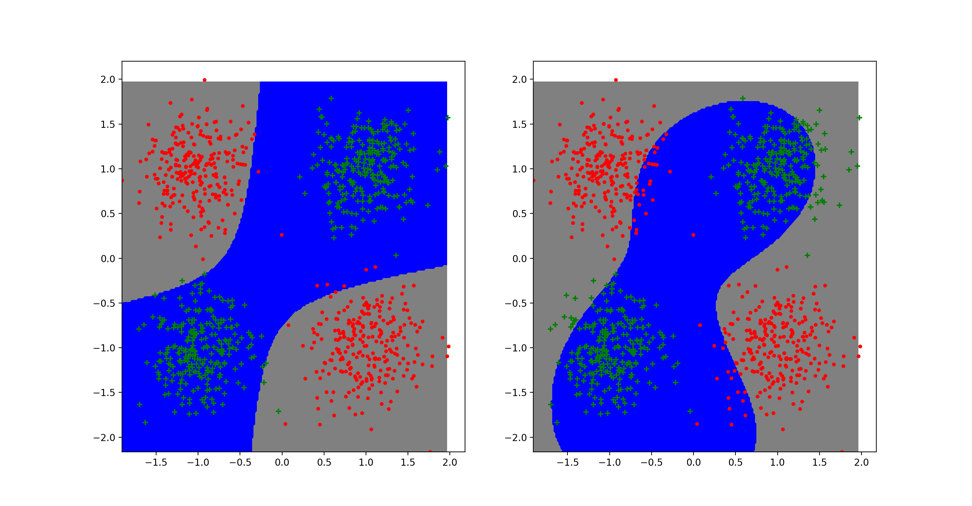
\includegraphics{Figures/Figure_10.png}
    	\caption{}
    	\label{WithProjection}
    \end{subfigure}
    \caption{Comparaison frontières de séparation de classes obtenues sans et avec des projections des données artificielles générées par \texttt{gen\_arti(nbex=1000, data\_type=1, epsilon=0.1)} : (a) -- sans projection, à gauche -- perceptron, à droite -- régression, (b) -- avec une projection, à gauche -- polynomiale, à droite -- gaussienne}
    \label{PolyGaussProjection}
\end{figure}

\section{TME 4 : SVM}
\label{tme4}

Dans le cadre de ce TME, l'on a appris une régularisation que l'on peut faire pour le perceptron. Par ailleurs, l'on a étudié comment est-ce qu'on peut utiliser le module \texttt{scikit-learn} afin d'entraîner nos modèles.

\textbf{Q 3.2.} Pour cette question l'on utilise une base de données \texttt{MNIST} qui stocke des chiffres manuscrites et qui est disponible depuis \texttt{tensorflow.keras.datasets.mnist.load\_data()}. Plus spécifiquement l'on a utilisé 8000 premiers exemplaires de l’échantillon d'apprentissage et 2000 de celui de test. Après avoir implémenté une version régularisée du perceptron, et après l'avoir lancée, on a une possibilité de la comparer avec les autres classificateurs. Ainsi, l'on a des scores suivants de bonne classification :

\begin{itemize}
    \item Perceptron simple : 91.5\%  pour apprentissage, 90.7\%  pour test ;
    \item Perceptron régularisé : 98.3\%  pour apprentissage, 96.6\%  pour test ;
    \item SVM : 99.8\%  pour apprentissage, 99\%  pour test.
\end{itemize}
En outre, des matrices de poids ainsi que l'évolution des erreurs sont fournies dans la Figure~\ref{PercRegRes}. Analysant tous ces résultats, l'on peut constater que le perceptron régularisé fait face au problème pour lequel on l'utilise : depuis la Figure~\ref{PercRegRes}, plus spécifiquement observant des matrices de poids, c'est clair que l'on traite des bruits dans les données de manière assez efficace. En plus, cette approche nous donne des meilleurs résultats que ceux du perceptron simple en termes de score de bonne classification. À l'inverse, SVM reste encore plus efficace garantissant le meilleur score parmi les algorithmes considérés.

\begin{figure}
    \centering
    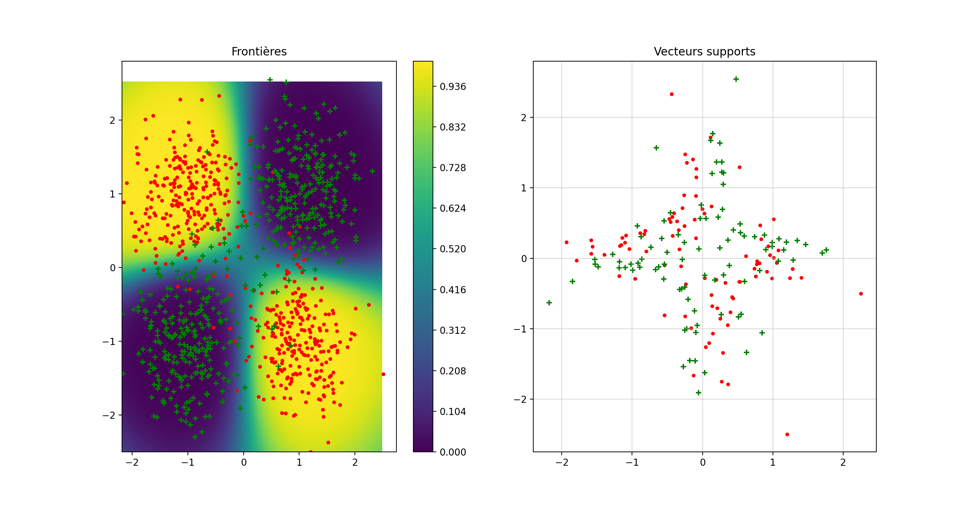
\includegraphics{Figures/Figure_14.png}
    \caption{Les résultats d'apprentissage de SVM sur les données artificielles dont les classes ne sont pas séparable linéairement}
    \label{SVMTest}
\end{figure}

\begin{figure}
    \centering
    \begin{subfigure}{1.0\textwidth}
    	\centering
    	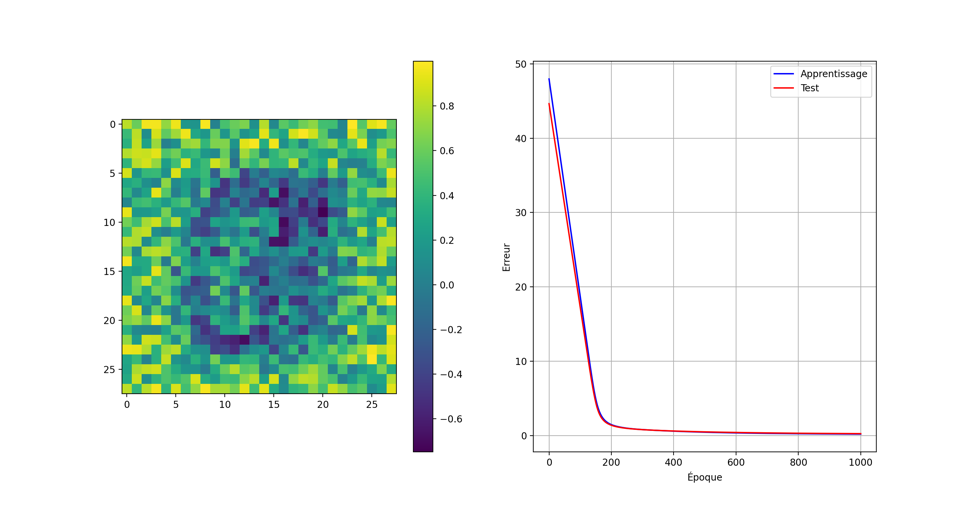
\includegraphics{Figures/Figure_11.png}
    	\caption{}
    	\label{PercNotRegRes}
    \end{subfigure}

    \begin{subfigure}{1.0\textwidth}
    	\centering
    	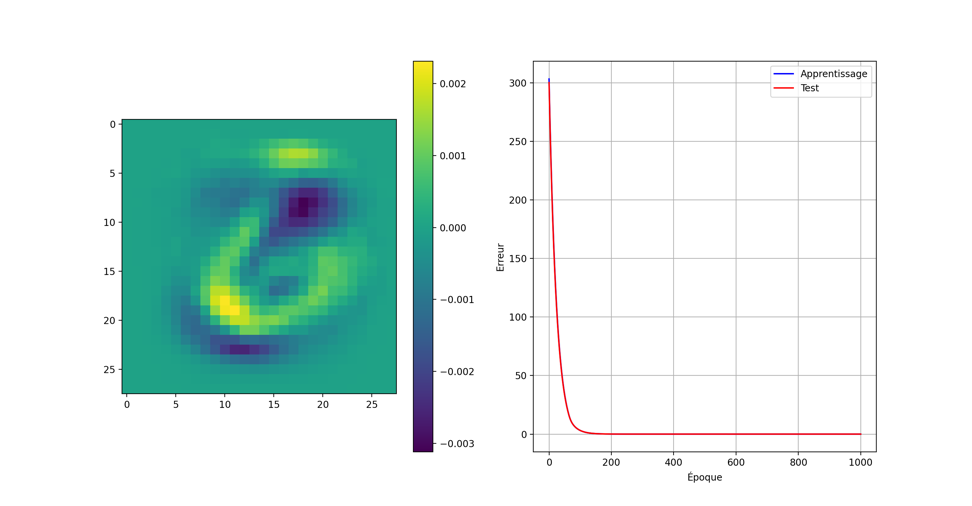
\includegraphics{Figures/Figure_12.png}
    	\caption{}
    	\label{PercIsRegRes}
    \end{subfigure}
    \caption{Les résultats obtenus pour l'apprentissage effectuée sur la base de données \texttt{MNIST} ; (a) -- Perceptron simple, (b) -- Perceptron régularisé}
    \label{PercRegRes}
\end{figure}

\textbf{Q 3.3.} L'on teste les fonctionnalités la SVM fournie par \texttt{scikit-learn} en la lançant sur les données artificielles générées par un appel \texttt{gen\_arti(nbex=1000, data\_type=1, epsilon=0.4} dont les classes ne sont pas séparables de manière linéaire. Ce n'est pas quand même le problème pour ce classificateur, comme l'on peut voir dans la Figure~\ref{SVMTest} et depuis le score de bonne classification qui a été égale à 95.4\% pour l'échantillon d'apprentissage, et 95.2\% pour celui de test.

La recherche dans une grille pour trouver des paramètres ``optimaux'' a été aussi réalisée et effectuée. L'on n'indique pas quand même ses résultats dans ce rapport pour des raison spatiales. Son implémentation se trouve dans un ficher \texttt{grid\_search.py}.

\textbf{Q 3.4.} L'on constate que \texttt{scikit-learn} fournit la possibilité de multi-classification utilisant des règles ``one-vs-one'' et ``one-vs-rest''. Choix d'une telle option s'effectue en passant une valeur correspondante au paramètre \texttt{decision\_function\_shape} au constructeur de SVM. L'on remarque qu'après avoir testé ces deux techniques pour multi-classification de chiffres de \texttt{MNIST} l'on obtient exactement les mêmes résultats tandis que ``one-vs-rest'' est plus efficace que ``one-vs-one'' en termes de ressources parce que dans tous les cas cela exige bien moins de classificateur à avoir. Par conséquent, l'utilisation de ``one-vs-rest'' est plus préférable.

\end{document}
